%%% FONT + LAYOUT %%%%%%%%%%%%%%%%%%%%%%%%%%%%%%%%%%%%%%%%%%%%%%%%%%%%%%%%%%%%
\documentclass[a4paper,11pt]{article}
\usepackage[T1]{fontenc} % ensures that ANSI carets and mid render correctly and are searchable

\usepackage{microtype}
\usepackage[mono=false]{libertine}
%\usepackage{beramono}
\usepackage[english]{babel}   % Spacing and hyphenation rules for English.

\usepackage[margin=25mm]{geometry}

\usepackage{calc}
\usepackage{xcolor}
\usepackage{graphicx}
\usepackage{verbatim}

% title
\usepackage{microtype}

%%% TITLE %%%%%%%%%%%%%%%%%%%%%%%%%%%%%%%%%%%%%%%%%%%%%%%%%%%%%%%%%%%%%%%%%%%%

\makeatletter
\renewcommand\maketitle{%
% main style
\pagestyle{fancy}
\fancyhead[L]{\@title}
\fancyhead[R]{\scshape Shtuka research}
\fancyfoot[L,C]{}
\fancyfoot[R]{\thepage}
\setlength{\headheight}{4ex}
\thispagestyle{plain}
\noindent\hrulefill

\vspace{5ex}

\noindent
\begin{minipage}{\textwidth * 3 / 4}
 {\noindent\Huge\scshape\color{darkgray}\textls*[50]{\@author}} \\
 \\
 {\noindent\Large\@title}
\end{minipage}%
% LOGO
\begin{minipage}{\textwidth / 4}
  \hfill
\includegraphics[height=10ex]{common/logo}
\end{minipage}

\vspace{5ex}

\noindent\hrulefill
}


\newcommand\maketitlepage{%
% main style
\pagestyle{fancy}
\fancyhead[L]{\@title}
\fancyhead[R]{\scshape Shtuka research}
\fancyfoot[L,C]{}
\fancyfoot[R]{\thepage}
\setlength{\headheight}{4ex}
\thispagestyle{plain2}
\quad\vfill
\noindent\hrulefill

\vspace{10ex}

\noindent
\begin{minipage}{\textwidth * 3 / 4}
 {\noindent\Huge\scshape\color{darkgray}\textls*[50]{\@author}} \\
 \\
 {\noindent\Large\@title}
\end{minipage}%
% LOGO
\begin{minipage}{\textwidth / 4}
  \hfill
\includegraphics[height=10ex]{common/logo}
\end{minipage}

\vspace{10ex}

\noindent\hrulefill
\vfill\newpage
}
\makeatother

%%% HEADERS %%%%%%%%%%%%%%%%%%%%%%%%%%%%%%%%%%%%%%%%%%%%%%%%%%%%%%%%%%%%%%%%%%

\usepackage{fancyhdr}

% plain style for first page
\fancypagestyle{plain}{%
  \fancyhf{}
  \fancyfoot[R]{\thepage}
  \setlength{\headheight}{4ex}
  \renewcommand\headrulewidth{0pt}
}


\fancypagestyle{plain2}{%
  \fancyhf{}
  \setlength{\headheight}{4ex}
  \renewcommand\headrulewidth{0pt}
}

% maths stuff

\usepackage{amsmath}
\usepackage{amsfonts}
\usepackage{amssymb}


%%% HYPERLINKS %%%%%%%%%%%%%%%%%%%%%%%%%%%%%%%%%%%%%%%%%%%%%%%%%%%%%%%%%%%%%%%

\usepackage[
  colorlinks=true,
  urlcolor=olive,
  linkcolor=teal,
  citecolor=olive,
  destlabel=true,
  bookmarks=true
]{hyperref}

% Turns cross-references into links by redefining \refstepcounter
% Turns citations into links by redefining \bibcite
% Turns amsmath equation numbers into links by unknown wizardry
% Provides \href{}{}

\usepackage{bookmark} 
% patches hyperref to simplify processing (no .out file is generated and 
% only needs 2 runs).
\usepackage{booktabs}
\urlstyle{same}

%%% amsthm configuration %%%%%%%%%%%%%%%%%%%%%%%%%%%%%%%%%%%%%%%%%%%%%%%%%%%%%

\usepackage{amsthm}

\swapnumbers        % Theorem number precedes heading.

% The following resets \end of theorem and proof environments to LaTeX
% defaults, which suppress indentation on immediately following line.

\usepackage{etoolbox}

\makeatletter
  \patchcmd{\@endtheorem}{\@endpefalse }{}{}{}
  \patchcmd{\endproof}{\@endpefalse}{}{}{}
\makeatother

% Initialize main counter
\newtheorem{paber@thm}{}[section]

% Theorem environment definitions
  \theoremstyle{plain}
    \newtheorem{theorem}[paber@thm]{Theorem}
    \newtheorem*{theorem*}{Theorem}
    \newtheorem{lemma}[paber@thm]{Lemma}
    \newtheorem*{lemma*}{Lemma}
    \newtheorem{proposition}[paber@thm]{Proposition}
    \newtheorem*{proposition*}{Proposition}
    \newtheorem{corollary}[paber@thm]{Corollary}
    \newtheorem*{corollary*}{Corollary}
  \theoremstyle{definition}
    \newtheorem{definition}[paber@thm]{Definition}
    \newtheorem*{definition*}{Definition}
    \newtheorem{question}[paber@thm]{Question}
    \newtheorem{question*}{Question}
  \theoremstyle{remark}
    \newtheorem{remark}[paber@thm]{Remark}
    \newtheorem*{remark*}{Remark}
    \newtheorem{example}[paber@thm]{Example}
    \newtheorem*{example*}{Example}

\newcommand\N{\mathbb{N}}
\newcommand\R{\mathbb{R}}
\newcommand\uR{\mathbb{R}_+}
\newcommand\Expectation{\mathbb{E}}
\newcommand\Prob{\mathbb{P}}

\newcommand\Mempool{\mathcal{M}}
\newcommand\Muxers{\mathcal{F}}
\newcommand\Builders{\mathcal{B}}
\newcommand\Accept{\alpha}
\newcommand\Safety{\mathbf{P}}

\newcommand\code[1]{{\color{darkgray}\texttt{#1}}}
%\newcommand\code[1]{\scalebox{0.7}[0.9]{\bfseries\color{darkgray}\texttt{#1}}}
% May also use [ttscale=0.9] in font package options

%%% BIBLIOGRAPHY %%%%%%%%%%%%%%%%%%%%%%%%%%%%%%%%%%%%%%%%%%%%%%%%%%%%%%%%%%%%%

\usepackage[style=numeric]{biblatex}
\setcounter{biburllcpenalty}{1}   % freely break URLs at lowercase

\usepackage{csquotes} % prevent a warning when using biblatex with babel

% exactly as misc but with doi and url fields removed
\DeclareBibliographyDriver{eprint}{%
  \usebibmacro{bibindex}%
  \usebibmacro{begentry}%
  \usebibmacro{author/editor+others/translator+others}%
  \setunit{\printdelim{nametitledelim}}\newblock
  \usebibmacro{title}%
  \newunit
  \printlist{language}%
  \newunit\newblock
  \usebibmacro{byauthor}%
  \newunit\newblock
  \usebibmacro{byeditor+others}%
  \newunit\newblock
  \printfield{howpublished}%
  \newunit\newblock
  \printfield{type}%
  \newunit
  \printfield{version}%
  \newunit
  \printfield{note}%
  \newunit\newblock
  \usebibmacro{organization+location+date}%
  \newunit\newblock
  \usebibmacro{eprint}%
  \newunit\newblock
  \usebibmacro{addendum+pubstate}%
  \setunit{\bibpagerefpunct}\newblock
  \usebibmacro{pageref}%
  \newunit\newblock
  \iftoggle{bbx:related}
    {\usebibmacro{related:init}%
     \usebibmacro{related}}
    {}%
  \usebibmacro{finentry}}
%


\addbibresource{../bib/pbs-builder-model.bib}

\author{Shtuka research}
\title{Report: Builder multiplexing in PBS}
\begin{document}
\maketitle

\section*{Background}

Concentration and exclusive `backroom deals' in Ethereum's PBS builder markets has long been a concern of the Ethereum blockspace community.
%
Concentration is regarded as an unwanted pathway to monopoly, centralisation, and all of the inefficiencies that entails. 
%
Unfortunately, it appears to be an inevitable consequence of the present structure of the blockspace supply chain that builders can only achieve edge by privately negotiated exclusive arrangements.
%
Worse than being simply opaque, exclusive arrangements are extremely hard to come by for new entrants and hence present an apparently insurmountable barrier to entry, severely limiting the competitiveness of builder markets.
%
Moreover, the exclusivity of these links fragments the market, reducing reliability.

In this work, we attempt to illuminate these issues by introducing an incentive model of builders and what we call \emph{multiplexers} or \emph{muxers}, that is, entities who forward transaction items to one or more builders together with a request for partial rebate.
%
The incentive model quantifies the tradeoff between the reliability of multiplexing to many builders and the possibility of obtaining a larger rebate from the edge that a single builder gains through an exclusive arrangement.
%
This builds on a body of previous work by quantifying at the model level:
%
\begin{itemize}
    \item \emph{why} order flow sources (OFS) might enter into risky exclusive arrangements, and 
    \item the conditions that make an OFS `pivotal' to a builder in the sense that its presence or absence decides the outcome of the PBS auction.
\end{itemize}
%
Finally, we wish to emphasise that our model assumes complete trust in the execution of the PBS auction.
%
The frictions we identify would therefore persist even if the well-known issue of trust in the relay were resolved.

\subsection*{Milestones}

The milestones of our original proposal were:
%
\begin{enumerate}
  \item 
    Develop preliminary supply side cost model for builder multiplexing. 
    %
    Incorporate tradeoff between OF inclusion risk, and value leakage to other builders and reduced win rate.

  \item
    Describe pathways to leverage the model to inform community decision-making.

  \item
    Scenario analysis: qualitative description of builder ``market power'' scenarios.
    %
    \begin{itemize}
      \item Do we expect small builders need to pay a larger percentage of their forwarded OF value to larger builders?
      \item Do we expect the forwarding price go up in rounds where a single builder dominates bidding (because of the latter's monopoly power)?
    \end{itemize}

\end{enumerate}

\subsection*{Key findings}

Our model predicts that PBS markets are dominated by builders with persistent edge, regardless of auction structure or profitability, and that the key sources of edge are OFS with high-value bundles and relatively high risk tolerance who may choose an exclusive forwarding strategy for its higher expected returns.
%
We find conditions under which exclusive flow can materialise even in the absence of a formal integration or `backroom deal' governing the relationship between the OFS and the builder.

Significantly, the model shows that this state of affairs --- already well known to be the case in the PBS market today --- is not due to the idiosyncracies of the present incumbents, the PBS auction rules, or the current reliance on trust in the execution of those rules.
%
Rather, it is an inevitable consequence of the single item auction structure of PBS and the existence of major OFS with certain risk preferences.

In more detail:
%
\begin{enumerate}
  \item 
    We describe the source of \emph{contention} between transaction items as a set of `safety rules' $\Safety$ on block construction.
    %
    As well as consensus rules, safety rules can be inherited from commitments further up the OF supply chain such as execution guarantees and bundle compatibility.
    
    By definition, contentious transactions are those for which inclusion into the optimal block depends on the other transactions in a builder's mempool.
    %
    It is therefore difficult to get strong upstream assurances about whether such items will be included.

  \item
    Builder muxing with nonzero rebate is a way for a builder to maintain edge at the same time as derisking by sharing flow.
    %
    Based on the current market layout, it appears that this edge is much smaller than those associated to exclusive flow.

  \item
    Market dominance in the current structure requires only consistent edge.
    %
    The size of the edge doesn't affect the amount of dominance.
    
    To allow builders with weaker edge to acquire non-trivial market share, a new market structure --- probably one with multiple sellers and multiple items --- is necessary.
    %
    Simply changing the auction format, as suggested in \cite{oz2024whoa}, isn't good enough.

  \item
    We identify two major theoretical sources of edge: originating contentious items (searcher-builder), and a preferential relationship on pivotal flows.
    %
    In the pivotal flows case, an exclusive forwarding strategy sometimes dominates even without a formal `backroom deal' or contention.
    %
    Even under conditions of complete trust in the PBS relay, these sources of edge are only available to builders with specific structural advantages or under specific builder market conditions.

  \item
    Once a builder has achieved market dominance, he can substantially increase his profit margins by making decisions on additional contentious items, including those where the contention is idiosyncratic to that builder (for example because of jurisdictional issues).
    %
    This single point of control over allocation is an efficiency and censorship threat.
\end{enumerate}


\subsection*{Recommendations for future research}

We call on the Ethereum research and business communities to intensify research into the following areas:
%
\begin{enumerate}
  \item
    \emph{Quantitative analysis of sources of builder edge.}
    %
    If the largest sources of edge were smaller, minor sources of edge like priority sharing could become viable routes to entry, improving market access.
    %
    To understand how these sources can be broken up and shared, we need a deeper, quantitative understanding of why exclusive arrangements of the two types identified are attractive for the OF sources.
    %
    This objective could be pursued with more detailed scenario analysis, gathering case studies, and statistical analysis of labelled data to fit the model parameters.

  \item
    \emph{Costs and returns of reliability guarantees.}
    %
    As far as we know there are currently no muxer services that offer a concrete guarantee on transaction landing rate.\footnote{Though Flashbots Protect does at least report theirs at \url{https://dune.com/flashbots/flashbots-protect}.}
    %
    For classes of items where contention is limited, more effort should be made into modelling landing rate with a goal of underwriting such a guarantee. 
    %
    Part of the work involved would be to explicitly identify the relevant low-contention classes.
    %
    Statistical research into the demand for improved reliability would illuminate the value of such constructions to the Ethereum business community.

  \item 
    \emph{Novel market structures for full blocks.} 
    The single change that we think would have the widest impact on the current bottlenecks of the PBS market would be to move from a single seller to multiple seller market for blocks, breaking the proposer monopoly on the single slot timescale.
    %
    Some movement in this direction is already under way, with partial block construction being factored out to other markets (via preconf protocols) or in-protocol committees (via FOCIL).
    
    Making this change for the full block, particularly the part of the block containing the highest value contentious items, would need either widespread community support for a consensus upgrade or a large fraction of validators signing up for an external commitment market.
    %
    We therefore expect this line of research to play out over a longer time scale than the previous two directions.
  
\end{enumerate}


%%%%%%%%%%%%%%%%%%%%%%%%%%%%%%%%%%%%%%%%%%%%%%%%%%%%%%%%%%%%%%%%%%%%%%%%%%%%%%


\section*{Model description}

We introduce a population $\Muxers$ of \emph{muxers} that receive transaction items from upstream \emph{clients} and forward them to other muxers or a second population $\Builders$ of \emph{builders}.
%
Builders aggregate items from the public mempool and from private flow, both direct and forwarded, and bid in a PBS auction to have their block added to the chain.

Compared to muxers, builders have several advantages:
%
\begin{enumerate}
  \item 
    Builders can decide the allocation of \emph{contentious items}, that is, contests where there are several items that cannot coexist in the same block.
    %
    Examples of contention are competitive trading opportunities (such as arb on large pools) attached to execution guarantees, multiple bundles containing the same transactions, and (rarely) congested blockspace.

  \item
    Builders receive the full transaction fee, rather than only a rebate.

\end{enumerate}
%
On the other hand, while muxers can gain high confidence of landing transactions by muxing to many builders, a builder runs a high risk of not winning the PBS auction and hence receiving a payout of zero.
%
To mitigate this risk, a builder may also function as a muxer, in which case he faces a tradeoff between reducing risk for his orderflow sources and increasing his opponents' chances to win the block auction.\footnote{A more commonly discussed strategy to increase landing rate is to subsidise one's own blocks by overbidding \cite{titan2023builder}.}

\subsection*{Strategies}

For each transaction item $\tau$ in the private mempool $\Mempool_i$ of a muxer $i$, $i$ must decide to which builders he will forward $\tau$ and what rebate $\sigma\in[0,1]$ he will request.
%
A muxer strategy is therefore a list of tuples $(\tau,\sigma,b)$ where $\tau\in\Mempool_i$, $\sigma\in[0,1]$, and $b\in\Builders$.

Builders move after receiving flow from muxers.
%
A builder strategy comprises the data of:
%
\begin{enumerate}
  \item a \emph{block} $B\in \mathrm{Block}(\mathcal{M}_b)$.

  The block $B$ is a finite, non-repeating sequence in $\mathcal{M}_b$ that may also need to follow some additional \emph{safety rules} $\Safety$.
  %
  A motivating example of a safety rule is that certain items in $\mathcal{M}_b$ may not be allowed to revert.

  \item A \emph{bid} $\beta>0$ for the PBS auction.
  \item 
    A set of \emph{accepted forwards} consisting of a muxer $i$, a transaction item $\tau\in B$, and a rebate rate $\sigma$.

    The idea is that a forward is an item $\tau$ that made it into the block after $b$ accepted it as forwarded private flow from $i$ with requested rebate rate of $\sigma$.
    %
    The fact that it was received in this manner entails an additional obligation on $b$, namely that it pay the rebate if it wins the block.

\end{enumerate}
%
A builder can define which forwards he will accept in advance by defining an \emph{acceptance policy} $\Accept(\sigma,\tau)$.
%
The acceptance decision for each forward may depend on the entire mempool state, not only on $(\sigma,\tau)$; in this case we say it is \emph{contentious}.
%
If an item $(i,\sigma,\tau)$ meets an acceptance criterion that depends \emph{only} on the transaction and rebate amount $(\sigma,\tau)$, it is non-contentious.



\subsection*{Outcomes}

An outcome $\omega = (W,B,\{(i,\tau,\sigma)\})\in \Omega_*$ consists of:
%
\begin{enumerate}
  \item 
    A builder $W\in\mathcal{B}$ (the \emph{winner});
  \item
    A \emph{block} $B\in \mathrm{Block}(\mathcal{M}_b)$;
  \item
    A set of \emph{forwards} consisting of a muxer $i$, a transaction item $\tau\in B$, and a rebate rate $\sigma$.
\end{enumerate}
%
The winner $W$ is determined by the set of bids $\{\beta_b\}_{b\in\Builders}$.

\subsection*{Payoffs}

The payoff of an outcome $(W,B,\{(i,\tau,\sigma)\})$ is determined as follows:
%
\begin{itemize}
  \item 
    The winner $W$ receives a gross revenue determined by the sum of the transaction fees in $B$, i.e.~$\sum_{\tau\in B}f(\tau)$.

    He must pay out his PBS bid $\beta$ plus a \emph{rebate} $\sigma\cdot f(\tau)$ to $i$ for each accepted forward $(i,\tau,\sigma)$.
  \item
    Each muxer $i$ receives the rebate $\sigma\cdot f(\tau)$ for each of his accepted forwards $(i,\tau,\sigma)$.
  \item
    All other builders receive nothing.
\end{itemize}
%
Expressed in formulas, we have:
%
\[
  U_b(b,B,\{(i,\tau,\sigma)\}) = \sum_{\tau\in B}f(\tau) - \beta - \sum_{(i,\sigma,\tau)}\sigma f(\tau)
\]
%
for the winning builder, and
%
\[
  U_i(W,B,\{(j,\tau,\sigma)\}) = \sum_{(j,\sigma,\tau), j=i}\sigma f(\tau)
\]
%
for a muxer $i$.
%
In the case of a muxer-builder, add these two terms; forwards from the builder to itself then cancel out of the expressions.

\subsection*{Value function}
Taking expectations over payoffs, we obtain
%
\[
  V_b = \Prob[\tilde{W}=b \mid \sigma] \cdot U_b(b,B,\{(i,\tau,\sigma)\})
\]
%
for a builder and 
%
\[
  V_i = \sum_{b\in\mathcal{B}} \Prob[\tilde{W}=b\mid\sigma]\cdot \sum_{(\tau,\sigma,b)}\Prob(\tilde\Accept_b(\sigma,\tau))\cdot\sigma f(\tau)
\]
%
for a muxer.
%
Note that the acceptance policy $\tilde\Accept_b$ may be, and in practice usually is, unknown, or at least depends on unknown covariates such as the presence of conflicting items in $\Mempool_b$.

For a muxer-builder, we find
\[
  V_b = \underbrace{\Prob[\tilde{W}=b \mid \sigma] \cdot U_b(b,B,\{(i,\tau,\sigma)\})}_{\text{builder}} + 
    \underbrace{\sum_{b'\in\Builders^\circ}\Prob[\tilde{W}=b' \mid \sigma] \cdot \sum\Prob(\tilde\Accept_{b'}(\sigma,\tau))\cdot\sigma f(\tau)}_{\text{muxer}}
\]


\subsection*{Risk}

A muxer $i$ faces the issue of managing the rate at which he lands his transactions $\tau\in\Mempool_i$.
%
If this rate is too low, he may find it difficult to attract customers to his unreliable service.
%
If he muxes his own transactions he may find it difficult to execute his strategies.

One way to approach this risk management matter is to model $i$'s decision process as constrained by the requirement that he must land private transactions $\tau\in\Mempool_i$ with probability at least $P_i\in[0,1]$. 
%
That is, $i$ must choose his strategy so that
%
\begin{align*}
  P_i &\leq \Prob(\tilde{W}=i \vee (\tilde{W}\neq i \wedge \Accept(\sigma,\tau))) \\
      &=    \Prob(\tilde{W}=i) + \sum_{b\in\mathcal{B}^\circ}\Prob(\tilde{W}=b)\cdot\Prob(\tilde\Accept(\sigma,\tau) \mid \tilde W=b) 
\end{align*}
%
for all $\tau$. 


\begin{remark*}[Portfolio management]

  The muxer-builder manages a cash-free portfolio of binary options.
  %
  \begin{itemize}
    \item Own flow $\tau$. Outcome is $f(\tau)$ if $i$ wins the PBS auction. Builder only.
    \item Forwarded flow $\tau_{\sigma\rightarrow b}$. Outcome is $\sigma f(\tau)$ if builder $b$ accepts the flow and wins PBS auction.
  \end{itemize}
  %
  We therefore wonder if the methods of portfolio management theory can usefully be applied to manage risk-reward tradeoffs.

\end{remark*}


%%%%%%%%%%%%%%%%%%%%%%%%%%%%%%%%%%%%%%%%%%%%%%%%%%%%%%%%%%%%%%%%%%%%%%%%%%%%%%


\section*{Discussion}


\subsection*{Scenario analysis}

We discuss here several muxer and muxer-builder strategies and the scenarios under which they become attractive.

    
\begin{comment}
\paragraph{Bid distributions}

\begin{itemize}
  \item
    If we model the PBS auction as an English auction (which is more or less accurate, except PBS bids may be cancelled), then for all non-winning bidders we should have $\tilde\beta \approx \tilde V_i(B_i)$, i.e.~their final bid is roughly the value of their best block.

  \item
    The value of the block is the sum of numerous (low hundreds) random components.
    %
    If we treat these components as independent and ignore mutual exclusivity rules about block construction, we posit that $V_i(B_i)$ follows a stable distribution.
    
  \item
    For any builder, the probability to win is an order statistic of the $\tilde V_i$s.

  \item
    Following \cite{titan2023builder}, we divide builders into \emph{leaders} (in reality, these are Titan and beaverbuild), \emph{midfield} (rsync-builder, BuilderNet, a few others), and \emph{long-tail}.

\end{itemize}
\end{comment}

\paragraph{Builder strategy}
%
Make the following simplifying assumptions about builder strategies:
%
\begin{enumerate}
  \item
    Builders bid according to the dominant strategy of an English auction with infinitesimal bid increments.
    %
    The winning bid is therefore equal to the value of the second most valuable block (net of rebates) at the end of the bidding period.

  \item
    Every builder $b$ has access to a `generalised knapsack oracle' that yields the optimal solution to the problem of building a value-maximising block from $\Mempool_b$ subject to safety rules $\Safety$.
\end{enumerate}
%
These assumptions completely determine builder strategy.
%
Outcomes then become a question of the structure of the $\Safety$-constrained optimisation problem of $\Mempool_b$ for each $b\in\Builders$.
%
Maximising builder revenue is then all about enlarging $\Mempool_b$, and edge is about enlarging it with items not visible to competitors.
%
Correspondingly, muxer strategy becomes about influencing builder behaviour and success rate by managing the population of $\Mempool_b$.

We remind the reader here that since PBS market share is usually measured in terms of PBS auction win rate, the size of builder edge --- that is, margin by which it wins the slots that it wins --- is completely irrelevant to market share. 
%
Only the proportion of times that it exceeds the edge of other builders is pertinent.
%
In particular, a builder that is consistently behind another builder, even by a tiny amount, will have $0\%$ market share.
%
By the revenue equivalence theorem of mechanism design, this is a byproduct of the single item, single seller market structure of PBS, and little to do with the particulars of the auction mechanism.

\paragraph{Contention}
%
If an item $(\tau,\sigma)$ is not likely to trigger any of the safety rules $\Safety$, it is non-contentious --- the decision on whether or not to include $(\tau,\sigma)$ has no impact on the strategy space of blocks on the remaining transactions.
%
Correspondingly, it is reasonable to expect that such items are included on a posted price basis as in \cite{roughgarden2021transaction}.

For contentious items, from the perspective of a muxer the acceptance probabilities $\Prob(\tilde\alpha_b(\sigma,\tau))$ may be relatively low, even when $\sigma$ is close to zero. 
%
In effect, the muxer faces a combinatorial auction over each point of contention.
%
A consequence of this is that under the current market structure there is no way to get ``telco-grade'' highly reliable landing assurances on such flow.

Acceptance probabilities for contentious items may be higher for weaker builders who have fewer conflicting items in their mempool.
%
Thus a strategy of muxing to a larger number of builders may be attractive in the contentious case.

\paragraph{Muxer strategies}
%
The basic muxer strategy is to derisk inclusion by forwarding items to all major builders.
%
As of 2023, most searchers do this \cite{titan2023builder}.

At the opposite extreme, we have the \emph{exclusive} strategy of forwarding to just one builder.
%
This strategy may be attractive when the exclusivity allows the muxer to request a larger rebate.
%
This happens when the flow is \emph{pivotal} for the builder in the sense of \cite{yang2024decentralization}.

In terms of our model, let $(i,\tau_i,\sigma_i)$ be a high-value forwarded item.
%
The optimal acceptance rule for this item is
%
\[
  \hat{\alpha}_b(\tau_i,\sigma_i) \qquad \Leftrightarrow \qquad [V_b\mid\alpha_b(\tau_i,\sigma_i)] - [V_b\mid \neg \alpha_b(\tau_i,\sigma_i)] > 0
\]
%
We can get some indication of the likely crossover regions by finding conditions under which the differential with respect to rebate $\sigma$ is large.
%
Firstly, the choice of rebate has no effect on value if the item is not accepted, that is $\frac{\partial}{\partial\sigma_i}[V_b\mid \neg \alpha_b(\tau_i,\sigma_i)] = 0$.
%
Secondly, in the acceptance case we obtain:
%
\begin{align*}
  \frac{\partial}{\partial\sigma_i}[V_b\mid\alpha_b(\tau_i,\sigma_i)] &= 
    \frac{\partial}{\partial\sigma_i}\left[ \Prob[\tilde{W}=b]\cdot \sum_{(\tau,\sigma)}(1-\sigma)\cdot f(\tau) \right] \\
    &= \left(\frac{\partial}{\partial\sigma_i}\Prob[\tilde{W}=b]\right)\cdot \sum_{(\tau,\sigma)}(1-\sigma)\cdot f(\tau)  - 
    \Prob[\tilde{W}=b]\cdot f(\tau_i) < 0.
\end{align*}
%
Here the bid $\beta$ drops out of the equation because at equilibrium it equals the value of the second most valuable block, which when an exclusive forwarding strategy is used does not depend on $\sigma_i$.
%
This quantity is large (and negative) when either $f(\tau_i)$ or $\frac{\partial}{\partial\sigma_i}\Prob[\tilde{W}=b]$ is large.
%
The second case is that of pivotal flow.
%
Note that if a sharing strategy is used, the choice of $\sigma$ does not affect any builder's net revenue; that is, $\frac{\partial}{\partial\sigma_i}[V_b\mid\alpha_b(\tau_i,\sigma_i)]=0$.

Even in such cases, any exclusive strategy is unlikely to achieve very high ($>99\%$) chance of success, so this approach works best when the muxer's clients have a high risk tolerance.
%
We expect Telegram bots and other retail-facing trading interfaces to be key examples.

\begin{figure}
    \begin{center}
        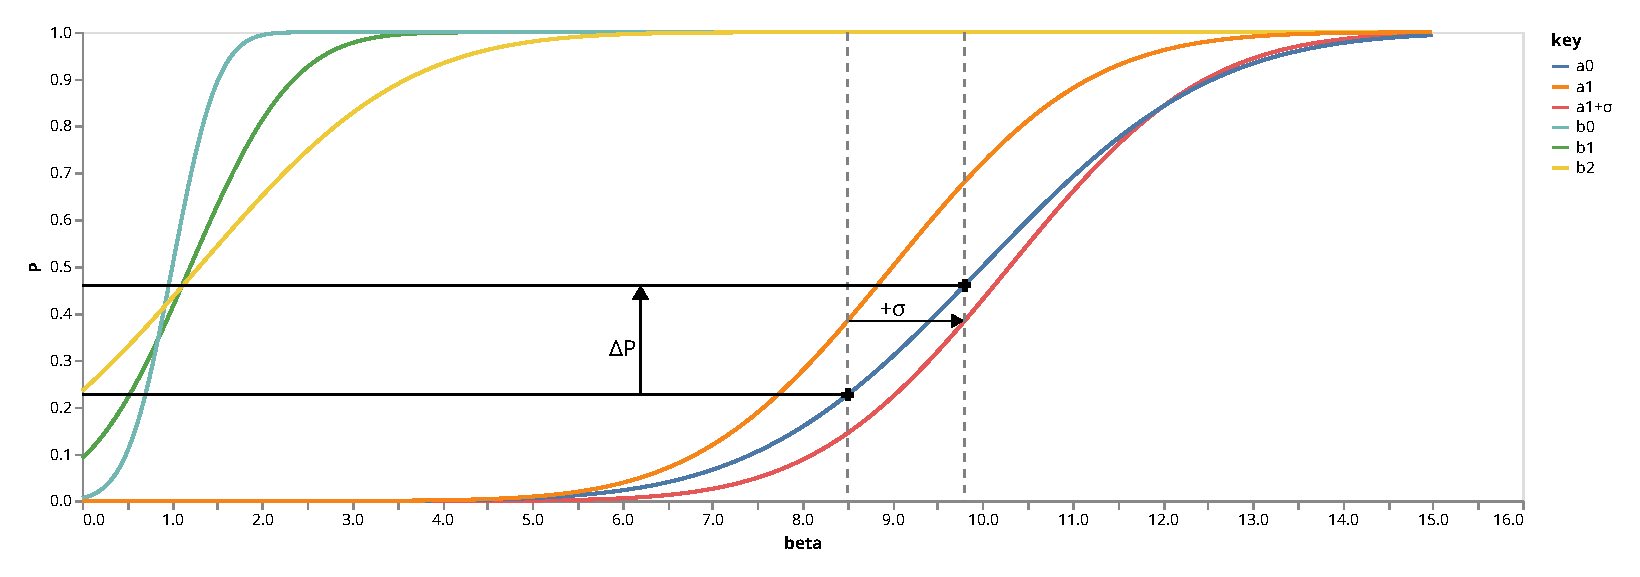
\includegraphics[width=0.8\textwidth]{eps/pivotal}
        \caption{CDFs of block values from a synthetic builder population with two major and a few long-tail builders. Values are normally distributed with a cutoff at zero.}
    
        \label{fig:pivotal}
    \end{center}
    
\end{figure}

\begin{example*}


In Figure \ref{fig:pivotal}, builder $a1$ draws a value of $8.5$ without $(\tau,\sigma)$.
%
By including the forward, his value jumps to $9.8$.
%
To find his chance of winning against the higher EV builder $a0$ at each point, follow the vertical line to the corresponding CDF graph.
%
The effect on $\Prob[\tilde{W}=b]$ of including $(\tau,\sigma)$ is 
\[
  \Delta P = F_{a0}(9.8)-F_{a0}(8.5) \approx 0.234.
\]
%
In other words, it more than doubles the chance of victory for $a1$.

\end{example*}

\paragraph{Extended builder strategies}
%
Builders face the choice of whether to accept items at cost (or opportunity cost in the case there are mutually exclusive items) or to try to elicit higher bids by credibly committing to an inflated reservation price. 
%
Even if there are major competitors with lower prices, risk-averse muxers may still wish to mux to the `premium' builder as well.
%
Perversely, the higher price then actually increases the premium builder's edge, giving him a higher win rate and increasing the value of forwarding flow to him.
%
It is not necessary to be a monopolist to pull this strategy off!


\paragraph{Muxer-builder strategies}

Clearly, if a muxer-builder uses an exclusive strategy then the receipient of the EOF is the integrated builder.
%
This is famously the situation for so-called HFT builders \cite{gupta2023centralizing}.
%
The flip side of this strategy is to insure the case where $b$ does not win the PBS auction by muxing to a selection of top and midfield builders.

\begin{remark*}

  If we assume no complementarity (i.e. all extractable value has already been bundled upstream), then forwarding with $\sigma=1$ should be strategically equivalent to not forwarding because the downstream builder derives no value from the forwarded flow.
  %
  We can therefore compare a non-forwarding strategy with one of forwarding with a large rebate by differential analysis as $\sigma=1$.

\end{remark*}

Inspecting the value function of the muxer-builder, one can see that value is maximised at $\sigma=1$ (i.e.~at the exclusive strategy) when all of the following are satisfied:
%
\begin{enumerate}
  \item
    $\Prob(\tilde\alpha_{b'}(\tau,\sigma))\cdot\sigma$ is small for all $\sigma$ --- in other words, $\tilde\alpha_{b'}(\tau,\sigma)$ is concentrated near $\sigma=0$ --- whence the muxer term of the value function is small and can be discarded.
  \item
    $\Prob(\tilde{W}=b\mid\sigma=1)$ is not too small.
\end{enumerate}
%
Again, this exclusive strategy works best for risk-neutral muxer-builders.
%
We expect the prototype case for this to be the builder with integrated CEX-DEX arbitrage strategy.

On the other hand, a risk-averse muxer-builder, or one with risk-averse upstream clients, may prefer to forward with $\sigma<1$ sooner (as $\Prob(\tilde{W}=b)$ gets smaller).
%
The prototypical example here is Flashbots Protect ``fast mode,'' as explained in their documentation.\footnote{\url{https://docs.flashbots.net/flashbots-protect/quick-start\#faster-transactions}}

\begin{remark*}
  
    A muxer-builder with zero market share (zero chance to win PBS auction) is roughly equivalent to a muxer. 
    %
    Strictly speaking, however, a builder incurs additional operational costs such as integrating with a MEV-Boost relay.

\end{remark*}


\paragraph{Cartelisation}

Muxer-builders also have a coalition strategy available: agree to forward certain private flow to each other, but not to builders outside the coalition.
%
As builders, coalition members should also agree not to bid away the value of these shared flows against one another, but to raise only against a non-member.
%
The space of strategies of how to manage redistribution among coalition partners seems not to have been explored in published research.

\subsection*{Real-world situation}

The two most prominent examples of services that fit into the mould of our model are Flashbots Protect and COWSwap's MEV-Blocker.\footnote{\url{https://orderflow.art/?isOrderflow=true&ofa=MEV+Blocker&ofa=Flashbots+Protect\&ofa=Flashbots+Protect+\%26+MEV+Blocker}}
%
In addition to muxing, both services provide additional features, most notably a backrun auction a.k.a.~OFA.\footnote{For a theoretical treatment of the OFA service, see also \cite{macpherson2024backrun}.}
%
Further examples are MeowRPC,\footnote{\url{https://meowrpc.com/}} Merkle,\footnote{\url{https://www.merkle.io/}} and Blink,\footnote{\url{https://docs.blinklabs.xyz/blink}} some of which also integrate OFAs.
%
Flashbots Protect is also integrated with Flashbots Builder; it is the prototypical example of our integrated muxer-builder.
%
It is also well-known that sophisticated users (i.e.~searchers) typically perform their own muxing \cite{titan2023builder}.

We also know \cite{yang2024decentralization} that in some special cases OF sources find it advantageous to submit to just one builder. 
%
Even when submitting to multiple builders, the trust requirements placed on the builder (i.e.~that they will not exploit the information contained in the forwarded flow) mean that many sources or muxers restrict the set of builders to whom they forward.

At time of writing, there is one (public) muxer-builder coalition in operation: BuilderNet.\footnote{\url{https://buildernet.org/docs/architecture}}

Although our model may seem to suggest that beginning life as a muxer offering low-risk transaction landing and jumping into block building after acquiring sufficient private flow may be a promising entry strategy for block builders, we don't know any real-world cases where this has happened.
%
We posit that this is because most of the flow valuable enough to be pivotal in PBS auctions is contentious, whence it hard for a muxer to get high confidence over the acceptance decision $\tilde\alpha_b$ without passing on unsustainably high fee bids.


\subsection*{Measurement}

Which quantities from this model can be measured?
%
\begin{enumerate}
  \item
    The probabilities $\Prob(\tilde{W}=b\mid \sigma)$ can be modelled using mechanism design methods. 
    %
    If the PBS auction is efficient --- we think this is a reasonable approximation --- the win probabilities are given by the CDF of an order statistic of the distribution of the net block value. 
    %
    The bids of non-winning bidders approximately equal their net block values.
    %
    These quantities can therefore be fitted using PBS bid history, which is publicly available from relay API endpoints.
    %
    The actual bidder strategies appearing in PBS auctions have been studied in some depth \cite{thierythomas2023empirical}.

  \item
    If rebate transactions can be linked to their parent transaction, rebate rates $\sigma$ can be observed.
    %
    In some cases, rebates occur during the same block.
    %
    Others, such as MEV-Blocker fees, are paid out of band; in this important case, the payment contract is public knowledge, so these rebates can also be tracked.
    %
    Measurement of $\sigma$ in general would probably require the use of specialised methods for each service.

  \item
    Even in the case that rebates can be tracked, we cannot generally observe rejected private transactions.
    %
    Making inferences about the acceptance rules $\tilde\alpha_b(\sigma,\tau)$ is therefore challenging.
    
    Separating OF types by label as in \cite{oz2024whoa}, we can try to estimate a `floor price' for each OFS.
    %
    If this floor price has high variability, the flow type may be contentious.


\end{enumerate}

\subsection*{Limitations}

\begin{itemize}
  \item The model does not take into account the possibility of multiple hop forwarding.
\end{itemize}


\newpage
\section*{Pathways to impact}

How can we leverage this model to influence how the Ethereum community builds?
%
We couch the discussion in terms of what we believe to be three core concerns: \emph{transparency}, \emph{centralisation vectors}, and \emph{reliability}.

\subsection*{Prior work}

\begin{itemize}
\item 
  In \cite{gupta2023centralizing}, a statistical model is used to find a relationship between price volatility, used as a proxy for CEX/DEX arbitrage opportunities, and dominance of so-called `HFT builders.'
  %
  Other OFS sources or features and alternative builder strategies are not considered.
  %
  Our model quantifies Remark 1 of \emph{op. cit}.

\item
  The article \cite{titan2023builder} uses a private dataset to illustrate the prevalence of multiplexing among searchers.

\item 
  The authors of \cite{oz2024whoa} perform extensive labelling of OFS, present visualisations on the breakdown of builder gross revenue, and computes Spearman correlations between profit margin and various OFS features.
  %
  The paper provides no opinion on methods to reduce the pivotal nature of exclusive as opposed to shared private orderflow.
  
\item
  \cite{yang2024decentralization} identifies the concept of pivotal flow.
  %
  The approach is combinatorial, focusing on identifying OFS whose inclusion or exclusion decides the game outcome, rather than quantitative.
  
  The proposed solution involves a centralised entity running a TEE, which is rather unsatisfactory from the perspective of resilience or censorship-resistance.
  
\end{itemize}


\subsection*{Transparency}

Publishing and disseminating insights into the structure and flows of the Ethereum blockspace supply chain improves trust and usability for broadcasters and builders alike.
%
Transparency lowers barriers to entry that have the form of information asymmetry. 
%
Smaller builders or broadcasters may enter the market with greater confidence about the competitive landscape, increasing competitiveness and hence improving services, diversity, and efficiency.

So far, the community has been successful in illuminating many facets of the PBS landscape:
%
\begin{itemize}
  \item The structure and cash flows of a subset of the OFA/muxer and builder relationships (excluding muxer-builders);
  \item The extent to which volatility, as a proxy for CEX/DEX arb value, drives builder profits;
  \item The breakdown of block revenue into components originating from various labelled OFS;
  \item Case studies and combinatorics of pivotal OFS in the current market;
  \item Partial data on transaction landing rates.
\end{itemize}
%
However, there is much more we could be doing via a combination of theory, publicly available data, and encouraging the publication of summaries of proprietary data:
%
\begin{itemize}
    \item 
      Further illuminate the strategy space.
      %
      Further exploration of the strategies of long tail and emerging `midfield' builders.
      %
       with a model-based approach by identifying strategies that are not currently being explored or exist under counterfactual scenarios;

      In-depth study entry strategies and complementarity (muxer-builder, searcher-builder). 
    \item 
      Identify common factors of the components that drive builder market share ranking \cite{oz2024whoa}, for example the relation to volatility \cite{gupta2023centralizing}.
      %
      Investigate the extent to which these factors drive builder \emph{net} revenue.
    \item 
      Further studies on landing rate and reliability, beyond Flashbots Protect.

      Can we uncover data on failures in exclusive flow strategies?
\end{itemize}

\subsection*{Builder centralisation}

The concerns of the community about concentration and entrenchment in the builder market can be understood in terms of multiple threats:
%
\begin{itemize}
    \item Monopolistic practices such as artificial scarcity and price hikes;
    \item Censorship,
    \item Other economic inefficiencies such as lack of investment into service improvements.
\end{itemize}
%
What does our model tell us about the severity of these threats and possible paths to resolution?
%
\begin{enumerate}
  \item 
    Does builder market concentration really cause these issues?
    %
    How centralised is too centralised? 
    %
    How about not centralised enough?
    
    By analogy with the model of \cite{chitra2024analysis}, entry costs are likely to be important drivers of the welfare-maximising answers to these questions.
    %
    As we have seen, entry costs are downstream of sources of edge and the risk appetites of OFS, so a model of these should help us understand the welfare of different concentration levels.

  \item
    Can we isolate centralisation threats by taking some responsibilities away from the builder?
    %
    For example, on a multi-block timescale, inclusion lists in Ethereum offload some allocation responsibility to a committee of validators.
    %
    On the single-block timescale, preconfirmation and similar commitment protocols may be able to do the same.
    
    To understand this we need a solid model of transaction contention and which types of flow it is feasible to push upstream.

  \item 
    How can anyone lower the barriers to entry to become a full block builder?
    
    Under the current market structure, we have seen that these barriers are driven by risk-tolerant, high value OFS.
    %
    Thus understanding the incentives of these sources is crucial to an investigation of what other structures might draw them away from exclusive builder arrangements.
    
    A more fundamental approach is to change the market structure of PBS by introducing multiple sellers.
    %
    Note that simply changing the \emph{auction format}, as proposed in \cite[\S6]{oz2024whoa}, does not solve this problem --- it is intrinsic to the single item, single seller auction.

\end{enumerate}

\begin{remark*}[A threat]

    Any approach the community takes to `democratise' or otherwise curtail specific sources of builder edge must be taken extremely carefully, for fear of collapsing the market into an even more fragile state.
    %
    For example, adopt the stylised model of the current market that Titan Builder's main source of edge is Telegram bot flow while beaverbuild's main edge is an integrated CEX/DEX arb searcher.
    %
    If the market structure changes in such a way as to break one of these sources of edge but not the other, the surviving builder could easily become a monopoly --- a far worse outcome than an apparently competitive duopoly.

\end{remark*}

\subsection*{Reliability}

A primary concern for the usability of Ethereum is its capacity to offer reliable assurances of inclusion and execution within specified time frames. 
%
For reasons illustrated by our model, the current system of builders and exclusive flow is not well-suited to provide that. 
%
Transaction originators wishing to avoid the public mempool must manage connection to multiple builders or delegate this responsibility to a downstream muxer.
%
No one is in a position to uphold a strong SLA for contentious items.

While much of the conversation around the problems facing the PBS market has focused on contention, there is much to be said for improving the reliability of Ethereum's handling of non-contentious, ordinary items. 
%
Important examples of low or no contention items are bridge locks and unlocks, rollup state root updates, and blobs. 
%
It's likely that these services can be improved substantially even without solving the harder issues.

How can the system deliver reliable service without breaching centralisation limits?
%
\begin{enumerate}
  \item Understand the rates at which contentious transactions land. Estimate the cost of landing transactions at different chance bounds on a per use case basis.
  \item Study mechanisms for coordinating acceptance decisions between builders for items falling under given constraints.
  \item Understand how important landing rate is to OFS. Study the relation between landing rate per service against demand growth.
\end{enumerate}
%


\appendix

\section*{Notation list}

\begin{itemize}
\item $\Muxers$ — muxer population
\item $\Builders$ — builder population
\item $i\in\Muxers$ — principal forwarder (optimiser)
\item $\Builders^\circ$ — non-principal builders
\item $\tilde{W}_t \stackrel{\$}{\in} \Builders$ — PBS auction winner 
\item $\beta$ — PBS auction bid
\item $\Mempool^\mathrm{pub}$ — public mempool
\item $\Mempool_i$ — private mempool of muxer $i$.
\item $\sigma$ — proportion of item fee to be refunded; $1/100$ times the value passed to \code{refundPercent} in the builder API.
\end{itemize} 

\printbibliography
\end{document}

